% Chapter Template

\chapter{Data Analysis and Pre-processing} % Main chapter title

\label{Chapter3}

%----------------------------------------------------------------------------------------
%	SECTION 1
%----------------------------------------------------------------------------------------

\section{Data labelling}

The first step is to generate the labels required to train the model.
Two different labels must be generated for each question we want to answer:

\begin{itemize}
    \item Remaining Useful Life (RUL) for the regression problem.
    \item Boolean flag indicating if the RUL is less than an specific cycle value.
\end{itemize}

%-----------------------------------
%	SUBSECTION 1
%-----------------------------------
\subsection{Remaining Useful Life}

In order to face the regression model to answer the question \textit{how many more cycles an in-service engine will last before it fails?} each entrance of the train dataset must include the number of remaining cycles until the aircraft fails.

This way, all the rows associated with the same aircraft identifier will have a decreasing number for this field. In the last step, where the cycle number represents the moment the aircraft fails, the RUL must be 0. See table \ref{tab:training-data-rul}

\begin{table}
\caption{Training Data with RUL column}
\label{tab:training-data-rul}
\centering
\begin{tabular}{l l l l l l l}
\toprule
\tabhead{Id} & \tabhead{Cycle} & \tabhead{Setting 1} & \tabhead{Setting 2} & \tabhead{S1} & \tabhead{...} & \tabhead{RUL}\\
\midrule
1 & 1   & -0.0007  & -0.0004 & 100.0 & ... & 191\\
1 & 2   & 0.0019   & -0.0003 & 100.0 & ... & 190\\
1 & 3   & -0.0043  & 0.0003  & 100.0 & ... & 189\\
... & ... & & & &  & ... \\
1 & 191 & 0        & -0.0004 & 100.0 & ... & 1\\
1 & 192 & 0.0009   & 0       & 100.0 & ... & 0\\
2 & 1   & -0.0018  & 0.0006  & 100.0 & ... & 286\\
2 & 2   & 0.0009   & -0.0003 & 100.0 & ... & 285\\
2 & 3   & 0.0018   & 0.0003  & 100.0 & ... & 284\\
... & ... & & & & & ... \\
\bottomrule\\
\end{tabular}
\end{table}

%-----------------------------------
%	SUBSECTION 2
%-----------------------------------

\subsection{Failure Cycle Window}

In the case of the binary classification model, the question to answer is \textit{is this engine going to fail within w1 cycles?}.

The w1 represents the window of cycles that we want to take in account to classify. In this dissertation the number of cycles will be set to 30.

Along with the RUL, it is possible to generate a label (label1) for each entrance indicating if the aircraft failed on this cycle window. To calculate it, just set to 1 ("true") all the RUL values lesser than w1. See table \ref{tab:training-data-w1}

\begin{table}
\caption{Training Data with label for classification}
\label{tab:training-data-w1}
\centering
\begin{tabular}{l l l l l l l l}
\toprule
\tabhead{Id} & \tabhead{Cycle} & \tabhead{Setting 1} & \tabhead{Setting 2} & \tabhead{S1} & \tabhead{...} & \tabhead{RUL} & \tabhead{label1}\\
\midrule
1 & 1   & -0.0007  & -0.0004 & 100.0 & ... & 191 & 0\\
1 & 2   & 0.0019   & -0.0003 & 100.0 & ... & 190 & 0\\
1 & 3   & -0.0043  & 0.0003  & 100.0 & ... & 189 & 0\\
... & ... & & & &  & & ... \\
1 & 191 & 0        & -0.0004 & 100.0 & ... & 1 & 1\\
1 & 192 & 0.0009   & 0       & 100.0 & ... & 0 & 1\\
2 & 1   & -0.0018  & 0.0006  & 100.0 & ... & 286 & 0\\
2 & 2   & 0.0009   & -0.0003 & 100.0 & ... & 285 & 0\\
2 & 3   & 0.0018   & 0.0003  & 100.0 & ... & 284 & 0\\
... & ... & & & & & & ... \\
\bottomrule\\
\end{tabular}
\end{table}

%----------------------------------------------------------------------------------------
%	SECTION 2
%----------------------------------------------------------------------------------------

\section{Feature Engineering and Normalization}

The information of the aircraft for each time step is formed by 21 different sensor and 3 setting numerical values.
The distribution of this values is shown in the figure \ref{fig:data-distribution}.

The data distribution shows that most of the sensor data follows a gaussian distribution, avoiding the existence of outliers. With this premise and also taking in account that some of the value ranges can take negative values, the normalization method chosen is min max scaler.

Min max scaler normalization transforms the values in the distribution to the range [0-1]. This normalization is required to avoid the network to priorize on features with higher values and also to avoid exploding gradient problems.

\begin{figure}[H]
    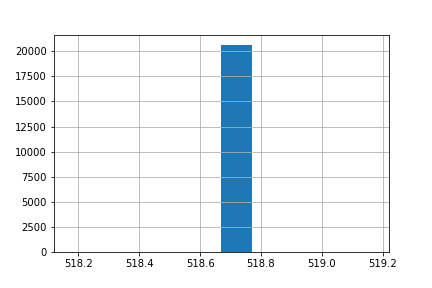
\includegraphics[width=.24\textwidth]{Figures/s1}\hfill
    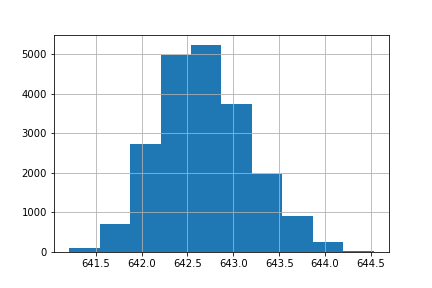
\includegraphics[width=.24\textwidth]{Figures/s2}\hfill
    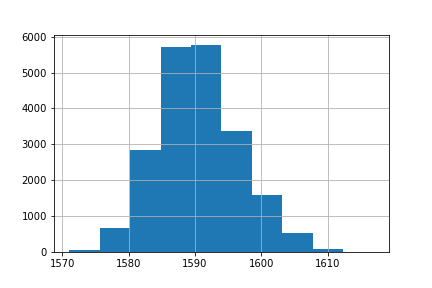
\includegraphics[width=.24\textwidth]{Figures/s3}\hfill
    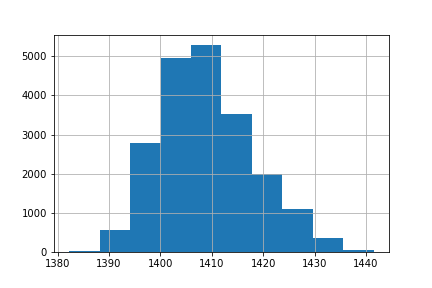
\includegraphics[width=.24\textwidth]{Figures/s4}
    \\[\smallskipamount]
    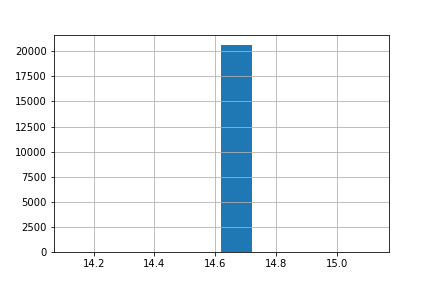
\includegraphics[width=.24\textwidth]{Figures/s5}\hfill
    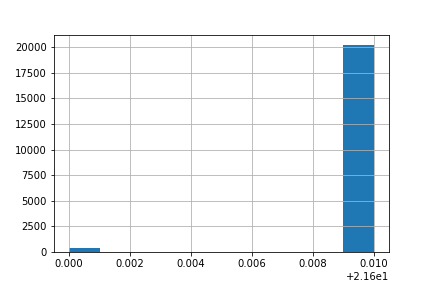
\includegraphics[width=.24\textwidth]{Figures/s6}\hfill
    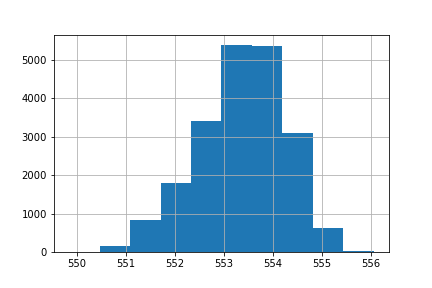
\includegraphics[width=.24\textwidth]{Figures/s7}\hfill
    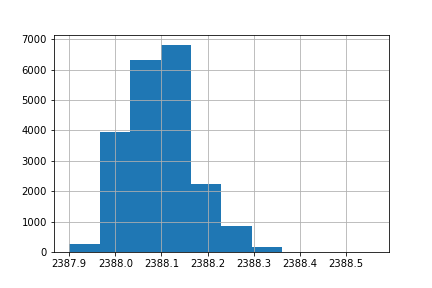
\includegraphics[width=.24\textwidth]{Figures/s8}
    \\[\smallskipamount]
    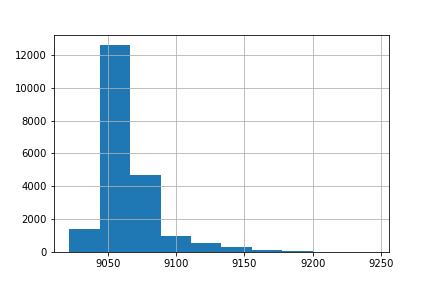
\includegraphics[width=.24\textwidth]{Figures/s9}\hfill
    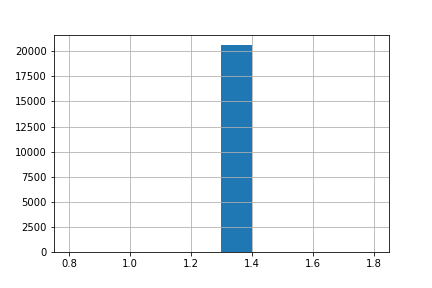
\includegraphics[width=.24\textwidth]{Figures/s10}\hfill
    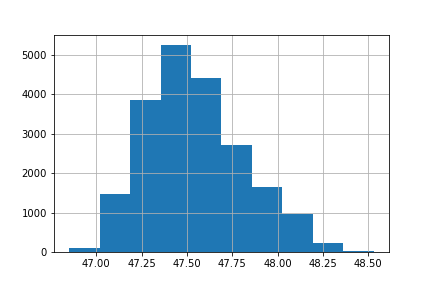
\includegraphics[width=.24\textwidth]{Figures/s11}\hfill
    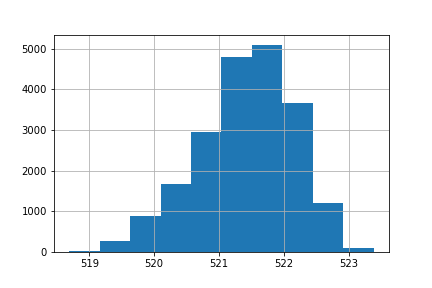
\includegraphics[width=.24\textwidth]{Figures/s12}
    \\[\smallskipamount]
    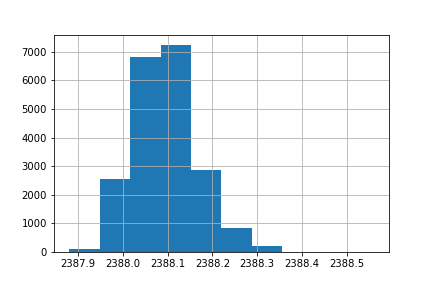
\includegraphics[width=.24\textwidth]{Figures/s13}\hfill
    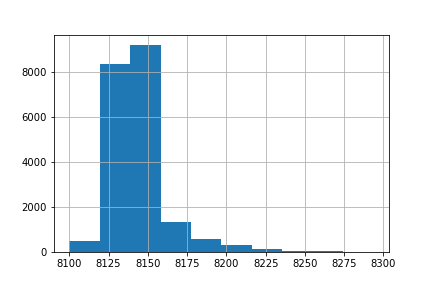
\includegraphics[width=.24\textwidth]{Figures/s14}\hfill
    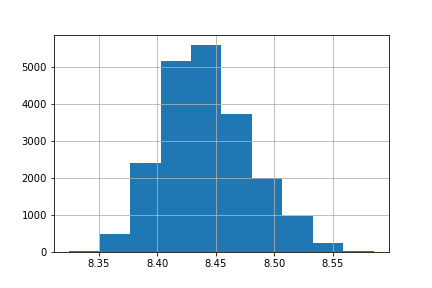
\includegraphics[width=.24\textwidth]{Figures/s15}\hfill
    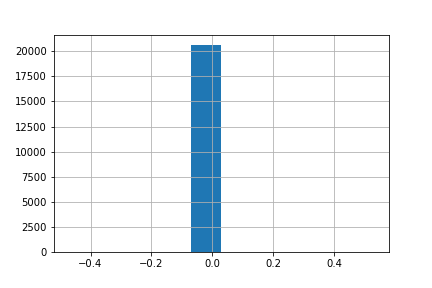
\includegraphics[width=.24\textwidth]{Figures/s16}
    \\[\smallskipamount]
    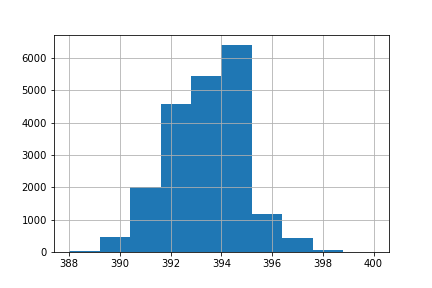
\includegraphics[width=.24\textwidth]{Figures/s17}\hfill
    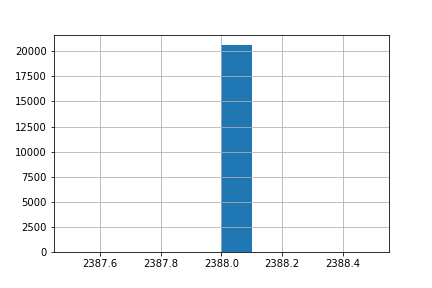
\includegraphics[width=.24\textwidth]{Figures/s18}\hfill
    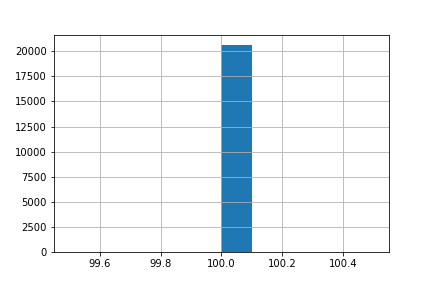
\includegraphics[width=.24\textwidth]{Figures/s19}\hfill
    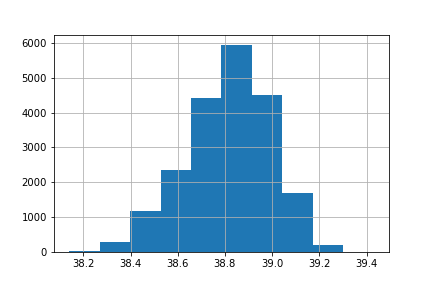
\includegraphics[width=.24\textwidth]{Figures/s20}
    \\[\smallskipamount]
    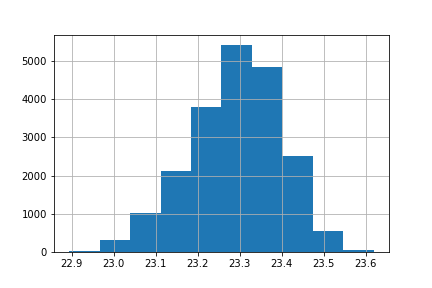
\includegraphics[width=.24\textwidth]{Figures/s21}\hfill
    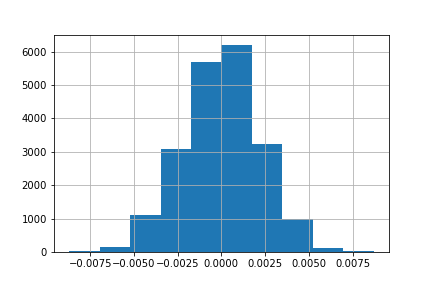
\includegraphics[width=.24\textwidth]{Figures/setting1}\hfill
    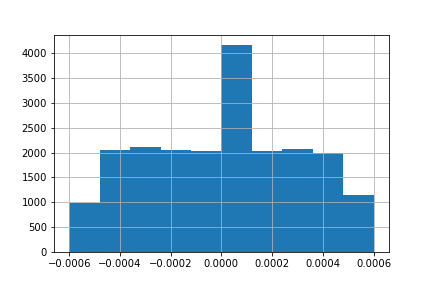
\includegraphics[width=.24\textwidth]{Figures/setting2}\hfill
    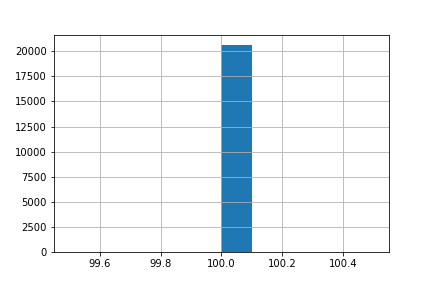
\includegraphics[width=.24\textwidth]{Figures/setting3}
    \caption{Sensor data distribution}\label{fig:data-distribution}
\end{figure}
